In this section, the required theoretical background and context for this thesis are explained. First, fundamental concepts of software development, the agile software development lifecycle (SDLC), Continuous Integration (CI), and software project hosting platforms are introduced. The second part explores Generative AI and LLMs with their rising role in software development practices. The third part examines the evolution and current state of Automated Program Repair (APR) with examples of existing approaches.

\section{Software Development}

The following section introduces core concepts of software development, starting with the software development lifecycle, followed by the importance of Continuous Integration (CI) in modern software development, and the role of software project hosting platforms.

\subsection{Software Development Lifecycle}
%TODO add tickets that are created by developers, product managers, ...
Engineering and developing software is a complex process, consisting of multiple different tasks. To structure this process, software development lifecycle models have been introduced. These frameworks constantly evolve to adapt to the changing needs of software creation. One of the most promising and widely used models today is Agile \cite{rupareliaSoftwareDevelopmentLifecycle2010, abrahamssonAgileSoftwareDevelopment2017}.

The Agile lifecycle introduces an iterative approach to software development, focusing on collaboration, feedback, and adaptability. The goal is frequent delivery of small functional software features, allowing continuous improvement and adaptation to changing requirements \cite{rupareliaSoftwareDevelopmentLifecycle2010, abrahamssonAgileSoftwareDevelopment2017}. Agile frameworks like Scrum or Kanban are used to apply this approach in a development environment \cite{zayatFrameworkStudyAgile2020}.

An Agile iteration consists of multiple stages. Figure \ref{fig:agile-cycle} shows an example of an agile iteration interpretation. Iterations start with a planning phase where requirements are gathered and prioritized. Secondly, the architecture and design of the required changes are constructed in the design phase. The third stage involves developing the prioritized requirements. After development, the changes are tested for issues or bugs in the testing stage. Upon successful integration and testing, the changes are released in the deployment stage. Finally, internal and user feedback is collected for review \cite{huoSoftwareQualityAgile2004}.

\begin{figure}[H]
    \centering
    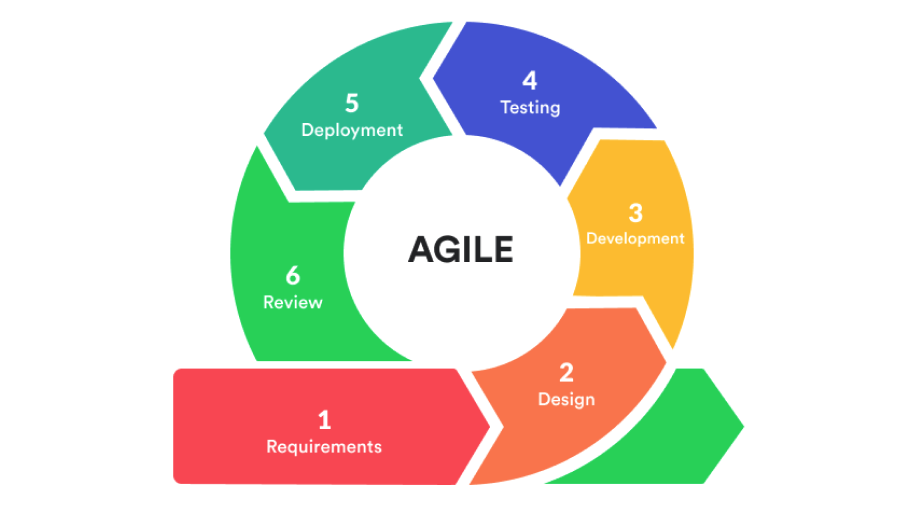
\includegraphics[width=1\textwidth]{images/agile-cycle.png}
    \caption{Agile software development lifecycle}
    \label{fig:agile-cycle}
\end{figure}

When bugs arise during an iteration, requirements can be reprioritized, and the iteration can be adapted to fix these issues. This adaptability is a key feature of Agile software development, allowing teams to quickly respond to changing requirements and issues that can slow down the delivery of planned features. %\cite{}. %TODO how do i cite this?

Modern software systems are moving towards loosely coupled microservice architectures, resulting in more repositories of smaller scale, tailored towards specialized domains. This trend is driven by the need for flexibility, scalability, and faster development cycles. This approach aligns with modern agile software development practices \cite{francescoResearchArchitectingMicroservices2017}. Along with this trend, developers tend to work on multiple projects simultaneously, which can lead to more interruptions and context switching when problems arise and priorities shift \cite{tregubovImpactTaskSwitching2017, vasilescuSkyNotLimit2016}.

\subsection{Continuous Integration}

Continuous Integration (CI) has become a standard practice in agile software development to accelerate software development and delivery. CI enables frequent code integration into a repository, automating steps like building and testing, thus providing rapid feedback right where the changes are committed. This supports critical aspects of agile software development, enhancing delivery, feedback, and collaboration \cite{ugwuezeContinuousIntegrationDeployment2024}. Figure \ref{fig:ci-cycle} illustrates a typical CI cycle, where code changes are automatically fetched from source control, built, and tested, with a report generated for the developer.

\begin{figure}[H]
    \centering
    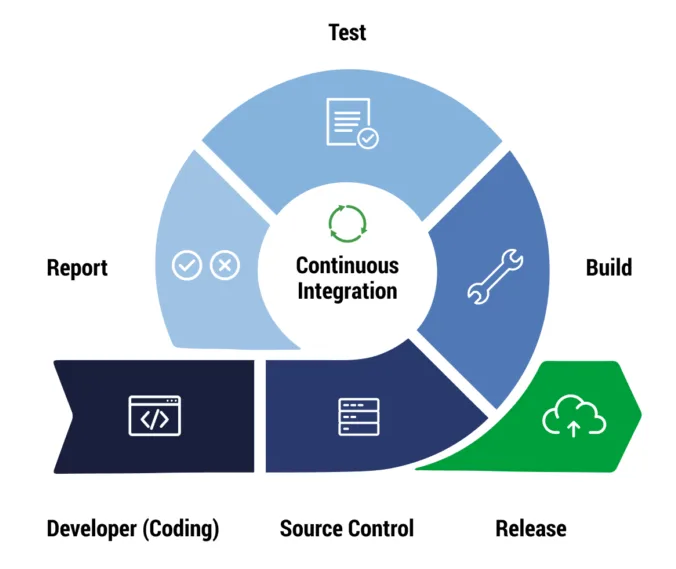
\includegraphics[width=1\textwidth]{images/ci-cycle.png}
    \caption{Continuous Integration cycle}
    \label{fig:ci-cycle}
\end{figure}

Although Continuous Integration improves feedback loops, it can also add overhead. Effort and infrastructure must be invested to keep pipelines running \cite{hiltonUsageCostsBenefits2016}, and projects may suffer from long build times that harm developer productivity \cite{ghalebEmpiricalStudyLong2019}.

\subsection{Software Project Hosting Platforms} \label{subsection:Software Project Hosting Platforms}

Modern software projects live on platforms like GitHub or GitLab. GitHub alone hosts 100 million developers and more than 518 million repositories, making it the largest open-source community worldwide \cite{staffOctoverseAILeads2024}.

Development platforms offer tools and services for the entire software development lifecycle, including project hosting, version control, issue tracking, bug reporting, project management, backups, collaborative workflows, and documentation capabilities \cite{GitHubFeatures2025, abrahamssonAgileSoftwareDevelopment2017}.

GitHub Issues are a key feature of GitHub, this feature enables project-scoped backlogs and tracking of tasks, features and bugs. Issues can be created, assigned, labeled, and commented on by everyone working on a codebase. This feature provides a structured way to manage and prioritize work within a project \cite{Issues}. Figure \ref{fig:gh-issue} shows an example of a GitHub Issue.

\begin{figure}[H]
    \centering
    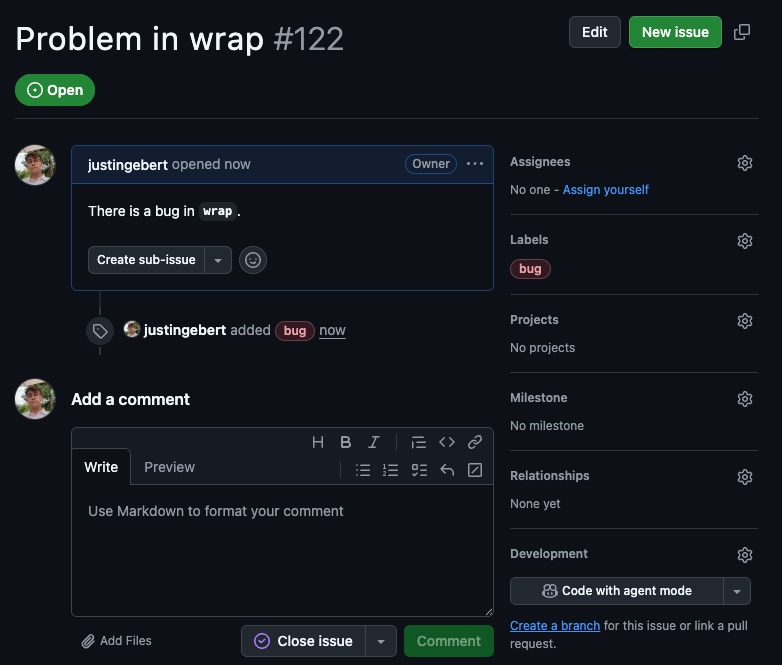
\includegraphics[width=1\textwidth]{images/github/github_issue.png}
    \caption{Example of a GitHub Issue}
    \label{fig:gh-issue}
\end{figure}

For integrating and reviewing code, GitHub uses Pull Requests. A Pull Request proposes changes to the codebase, integrating a review process to validate changes before merging into the production codebase. Code changes are displayed in a diff format \footnote{TODO explain format}, allowing reviewers to examine the changes made. This process is essential for maintaining code quality and ensuring that changes are validated before merging. Pull requests can be linked to Issues, allowing easy tracking of changes related to specific tasks or bugs \cite{PullRequests}.

Moreover, GitHub also provides a managed solution (GitHub Actions) for running CI pipelines in repositories. CI pipelines are configured by writing workflow files in YAML. Workflows can run self-hosted or hosted by GitHub. A workflow consists of triggers, jobs, and steps. One or more events trigger a workflow, which executes one or more jobs consisting of multiple steps \cite{UnderstandingGitHubActions}. Figure \ref{fig:gh-workflow} visualizes part of a workflow on GitHub.

\begin{figure}[H]
    \centering
    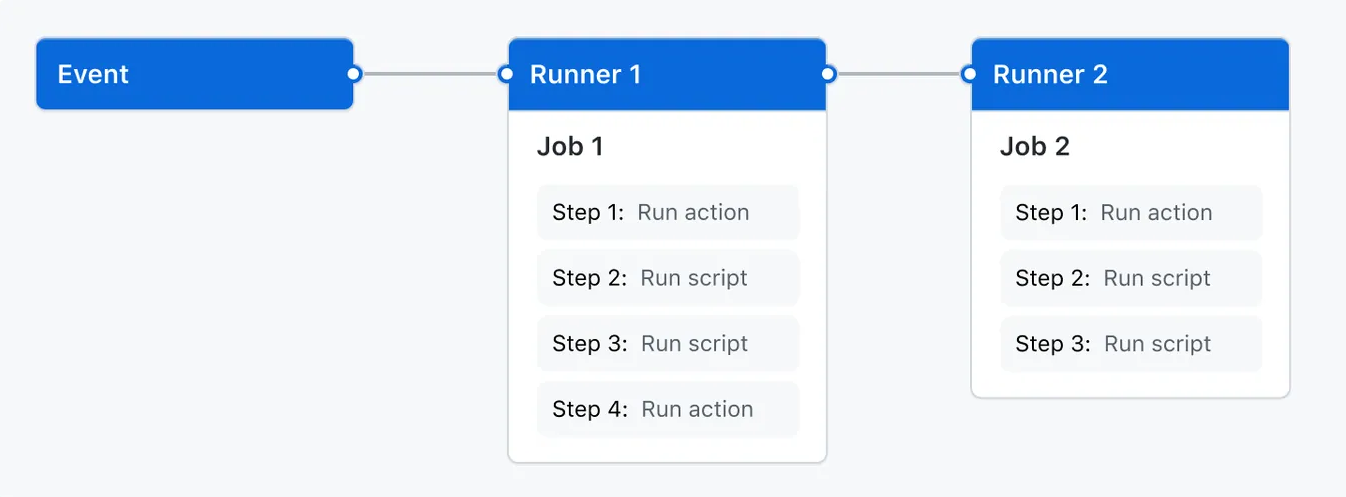
\includegraphics[width=1\textwidth]{images/overview-actions-simple.png}
    \caption{Components of a GitHub Action}
    \label{fig:gh-workflow}
\end{figure}

Workflow results and logs can be viewed from multiple places in the GitHub Web User Interface (UI), including the Actions tab, the Pull Request page, and the repository's main page. This integration provides a seamless experience for developers to monitor and manage their CI processes directly within their repositories \cite{GitHubActions2025}.


\section{Generative AI in Software Development}

This section covers the role of Generative AI in modern software development. First, Generative AI and Large Language Models (LLMs) are defined. The second part focuses on the impact of Generative AI on software development practices.

\subsection{Generative AI and Large Language Models}
%TODO add thinking definition of LLMS - and llms are few shot better than zero shot -> cite few shot learners paper
Generative Artificial Intelligence (GenAI) is a subfield of artificial intelligence referring to systems that generate new content based on patterns learned from extensive training data. Advanced machine learning techniques, particularly deep learning, enable these systems to generate text, images, or code that resembles human-generated output \cite{WhatGenerativeAI2021}.

The introduction of the transformer architecture revolutionized the field of text generation and natural language processing (NLP). This architecture laid the groundwork for Large Language Models \cite{changSurveyEvaluationLarge2024, naveedComprehensiveOverviewLarge2024}. Extensive training results in LLMs with billions of parameters, allowing them to understand and generate text in natural languages and diverse programming languages. Research has shown that a model's size impacts its performance, with larger models generally achieving better results in various NLP tasks \cite{kaplanScalingLawsNeural2020}. However, training and operating larger models require significant computational resources \cite{LLMsWhatsLarge, naveedComprehensiveOverviewLarge2024}. Furthermore, despite modern LLMs showing promising results in text generation, they can still hallucinate incorrect or biased content \cite{LLMsWhatsLarge}.

To achieve specific tasks using LLMs, an input prompt must be provided. Designing this input is a process known as prompt engineering. The quality and specificity of the prompt directly influence the model's output. In zero-shot prompting, the model is given only the task description, while in few-shot learning, a few relevant examples are included to better guide the model's behavior. Brown et al.~\cite{brownLanguageModelsAre2020} showed that few-shot prompting can remarkably improve model performance across diverse tasks.

Text used for input and output is tokenized, meaning the text is broken down into smaller units (tokens) for processing. The input is constrained by a model's context window, which is the maximum amount of text the model can process at once \cite{naveedComprehensiveOverviewLarge2024}.

Large Language Models can be accessed via APIs offered by providers like OpenAI, Anthropic, or Google. A selection of LLMs with characteristics is shown in section \ref{subsection:llm-selection}.

\subsection{Large Language Models in Software Development}

Large Language Models are reshaping software development by automating various tasks \cite{houLargeLanguageModels2024}. With billions of parameters and pre-training on massive codebases, these models exhibit extraordinary capabilities in this area \cite{chenUnveilingPitfallsUnderstanding2025}. Tools like ChatGPT\footnote{link to gpt} and GitHub Copilot\footnote{link to copilot} have become popular in the software development community, providing developers with AI-powered code suggestions and completions \cite{bhargavmallampatiRoleGenerativeAI2025}. These tools are applied in various stages of the software development lifecycle, including requirements engineering, code generation, refactoring, testing, and debugging \cite{houLargeLanguageModels2024, puvvadiCodingAgentsComprehensive2025, bhargavmallampatiRoleGenerativeAI2025}. By using LLMs, development cycle times can be reduced by up to 30 percent \cite{bhargavmallampatiRoleGenerativeAI2025, kalliamvakouResearchQuantifyingGitHub2022}. Furthermore, these tools positively impact developer satisfaction and reduce cognitive load \cite{kalliamvakouResearchQuantifyingGitHub2022}.

Despite the rapid adoption of Generative AI in many areas of software development, this technology still faces limitations. LLMs have difficulty with tasks outside their training scope or requiring specific domain knowledge \cite{houLargeLanguageModels2024}. Limited context windows create challenges when working with large codebases and complex projects, restricting true contextual or business requirement understanding \cite{bhargavmallampatiRoleGenerativeAI2025}. When generating code, LLMs can produce incorrect or insecure outputs, leading to additional bugs and vulnerabilities \cite{houLargeLanguageModels2024, bhargavmallampatiRoleGenerativeAI2025}. Additionally, integrating LLMs can introduce vulnerabilities to prompt injection, where malicious instructions lead to harmful code generation \cite{liuPromptInjectionAttack2024}. Moreover, code generated by LLMs is based on existing training data, raising questions about ownership, responsibility, and intellectual property rights \cite{sauvolaFutureSoftwareDevelopment2024, houLargeLanguageModels2024}.

Facing these challenges, different approaches are actively being developed and researched, including AI Agents \cite{liuMarsCodeAgentAInative2024, yangSWEagentAgentComputerInterfaces2024}, Retrieval Augmented Generation (RAG) approaches \cite{xiaAgentlessDemystifyingLLMbased2024}, and interactive systems \cite{xiaAutomatedProgramRepair2024}. These paradigms aim to enhance LLM capabilities by providing additional context, enabling multi-step reasoning, or allowing interactive feedback loops during code generation and debugging \cite{houLargeLanguageModels2024, puvvadiCodingAgentsComprehensive2025}. Section \ref{subsection:evolution-apr} discusses these approaches in more detail.

Recent research is exploring solutions integrating LLMs into existing software development practices and workflows, leveraging existing development tools and platforms for seamless integration into the software development lifecycle \cite{puvvadiCodingAgentsComprehensive2025, dohmkeGitHubCopilotMeet2025, IntroducingCodex, sauvolaFutureSoftwareDevelopment2024}.

\section{Automated Program Repair}

Automated Program Repair (APR) describes software used to detect and repair bugs in codebases with minimal human intervention \cite{zhangSurveyLearningbasedAutomated2024}. APR aims to automate the bug-fixing process, reducing workload for developers and allowing them to focus on more relevant tasks \cite{houLargeLanguageModels2024}.

APR systems fix specific bugs by applying patches, typically generated using a three-stage approach: first localizing the bug, then repairing it, and finally validating the fix \cite{zhangSurveyLearningbasedAutomated2024, baderGetafixLearningFix2019}. This approach mirrors a developer's bug-fixing process, where the bug is identified, fixed, and then tested and reviewed to ensure the fix works as intended \cite{yangSWEagentAgentComputerInterfaces2024}. GetaFix \cite{baderGetafixLearningFix2019} is a prominent example of an APR system applied at scale, used at Meta to automatically fix common bugs in their production codebases.

The field of APR has greatly benefited from rapid advancements in AI and ML, with new research and benchmarks continually setting higher standards \cite{puvvadiCodingAgentsComprehensive2025, houLargeLanguageModels2024}.

This section provides an overview of the evolution of APR, related work, and the current state of APR systems, followed by a selected list of common APR benchmarks used in research and industry.

\subsection{Evolution of Automated Program Repair} \label{subsection:evolution-apr}

Automated Program Repair has experienced multiple paradigm shifts over the years, categorized into key stages marked by significant advancements in techniques and methodologies.

\textbf{Traditional Approaches:}

Traditional APR approaches typically rely on manually crafted rules and predefined patterns \cite{liuMarsCodeAgentAInative2024, xiaAutomatedProgramRepair2023, yinThinkRepairSelfDirectedAutomated2024}. These methods can be classified into three main categories: search-based, constraint/semantic-based, and template-based repair techniques.

\begin{itemize}
    \item \textbf{Search-based repair} searches for the correct predefined patch within a large search space \cite{liuMarsCodeAgentAInative2024, huCanGPTO1Kill2024, zhangPATCHEmpoweringLarge2025}. A popular example is GenProg, which uses genetic algorithms to evolve patches by mutating existing code and selecting patches based on fitness determined by test cases \cite{legouesGenProgGenericMethod2012}.

    \item \textbf{Constraint/Semantic-based repair} synthesizes patches using constraint solvers derived from the program's semantic information and test cases \cite{liuMarsCodeAgentAInative2024, mechtaevAngelixScalableMultiline2016}. Angelix is a prominent example of this approach \cite{mechtaevAngelixScalableMultiline2016}.

    \item \textbf{Template-based repair} relies on mined templates for transformations of known bugs \cite{xiaAutomatedProgramRepair2023}. These templates are mined from previous human-developed bug fixes \cite{xiaAutomatedProgramRepair2023, yinThinkRepairSelfDirectedAutomated2024}. GetaFix is an industrially deployed tool, learning recurring fix patterns from past fixes \cite{baderGetafixLearningFix2019}.
\end{itemize}

These traditional approaches face significant limitations in scalability and adaptability. They struggle to generalize to new and unseen bugs or adapt to evolving codebases, often requiring extensive computational resources and manual effort \cite{puvvadiCodingAgentsComprehensive2025, xiaAutomatedProgramRepair2024}.

\textbf{Learning-based Approaches:}

Machine learning techniques introduced learning-based APR, increasing the variety and number of bugs that can be fixed. Deep neural networks leverage bug-fixing patterns from historical fixes as training data to learn how to generate patches and translate buggy code into correct code \cite{xiaAutomatedProgramRepair2023, tangLargeLanguageModels2024}. Prominent examples include CoCoNut \cite{lutellierCoCoNuTCombiningContextaware2020} and Recoder \cite{zhuSyntaxguidedEditDecoder2021}. Despite significant advancements, these methods remain limited by training data and struggle with unseen bugs \cite{xiaLessTrainingMore2022}.

\textbf{The Emergence of LLM-based APR:}

The recent rapid growth of LLMs has transformed the APR field. LLM-based APR techniques demonstrate significant advancements over traditional state-of-the-art techniques, leveraging the advanced code-generation capabilities of modern LLMs \cite{hossainDeepDiveLarge2024}. Consequently, LLMs form the foundation of a new APR paradigm \cite{chenUnveilingPitfallsUnderstanding2025, anandComprehensiveSurveyAIDriven2024}.

Different LLM-based approaches have emerged and are actively researched, categorized into four main paradigms:

\begin{itemize}
    \item \textbf{Retrieval-Augmented approaches} enhance bug repair by retrieving relevant context, such as code documentation stored in vector databases, during the repair process \cite{puvvadiCodingAgentsComprehensive2025}. This approach allows access to external knowledge, enhancing LLMs' bug-fixing capabilities \cite{houLargeLanguageModels2024, yinThinkRepairSelfDirectedAutomated2024}.

    \item \textbf{Interactive/Conversational approaches} utilize LLMs' dialogue capabilities, providing instant developer feedback during patch validation \cite{xiaAutomatedProgramRepair2024, huCanGPTO1Kill2024}. This iterative feedback loop refines generated patches to achieve better outcomes \cite{xiaAutomatedProgramRepair2024}.

    \item \textbf{Agent-based approaches} enhance bug localization and repair by equipping LLMs with the ability to access external environments, operate tools (e.g. file editors, terminals, web search engines), and make autonomous decisions \cite{anandComprehensiveSurveyAIDriven2024, puvvadiCodingAgentsComprehensive2025, mengEmpiricalStudyLLMbased2024}. Using multi-step reasoning, these frameworks replicate developers' cognitive processes through specialized agents \cite{rondonEvaluatingAgentbasedProgram2025, zhangPATCHEmpoweringLarge2025, leeUnifiedDebuggingApproach2024}. Examples include SWE-Agent \cite{yangSWEagentAgentComputerInterfaces2024}, FixAgent \cite{leeUnifiedDebuggingApproach2024}, MarsCodeAgent \cite{liuMarsCodeAgentAInative2024}, and GitHub Copilot \cite{dohmkeGitHubCopilotMeet2025}.

    \item \textbf{Agentless approaches} focus on simplicity and efficiency, reducing complex multi-agent coordination while maintaining effectiveness \cite{xiaAgentlessDemystifyingLLMbased2024, puvvadiCodingAgentsComprehensive2025}. These approaches provide clear guardrails for LLMs, improving transparency. The three-step approach (localization, repair, validation) of Agentless approaches achieves promising results at low cost \cite{xiaAgentlessDemystifyingLLMbased2024, mengEmpiricalStudyLLMbased2024}.
\end{itemize}

Popular LLMs for APR include ChatGPT, Codex, CodeLlama, DeepSeek-Coder, and CodeT5 \cite{houLargeLanguageModels2024, yinThinkRepairSelfDirectedAutomated2024, anandComprehensiveSurveyAIDriven2024}. Despite the significant advancements brought by LLMs, state-of-the-art APR systems continue to face notable challenges and limitations. Existing systems are often complex, with limited transparency and control over the bug-fixing process \cite{xiaAgentlessDemystifyingLLMbased2024, puvvadiCodingAgentsComprehensive2025, houLargeLanguageModels2024}. Additionally, the repairs are computationally intensive and time-consuming, leading to high costs \cite{sobaniaAnalysisAutomaticBug2023, puvvadiCodingAgentsComprehensive2025}.
Furthermore a barrier to practical adoption remains: most APR systems are developed and evaluated in controlled environments. Consequently, there is still a lack of research and experience on integrating these approaches into real-world software development workflows and projects \cite{meemExploringExperiencesAutomated2024, puvvadiCodingAgentsComprehensive2025}.


\subsection{APR Benchmarks}

To standardize the evaluation of new APR approaches, benchmarks have been developed. These benchmarks consist of software bugs and issues, along with their corresponding fixes or tests, which can be used to evaluate the effectiveness of different APR techniques \cite{anandComprehensiveSurveyAIDriven2024}. They are essential for comparing the performance of different APR systems and for understanding their strengths and weaknesses \cite{puvvadiCodingAgentsComprehensive2025}. APR benchmarks are available for various programming languages, with a selection of popular benchmarks listed in \ref{table:benchmarks} \cite{wangSoftwareDevelopmentLife2025}.

\begin{table}[ht]
    \centering
    \small
    \renewcommand{\arraystretch}{1.5}
    \begin{tabular*}{\textwidth}{@{\extracolsep{\fill}} p{2.8cm} | p{2.8cm} | p{2.8cm} | p{5cm}  @{}}
        \hline
        \textbf{Model} & \textbf{Languages} & \textbf{Number of Bugs} & \textbf{Description}  \\
        \hline
        QuixBugs \cite{linQuixBugsMultilingualProgram2017} & Python, Java & 40 & small single line bugs  \\ \hline
        Defects4J \cite{justDefects4JDatabaseExisting2014} & Java & 854 & real-world Java bugs  \\ \hline
        ManyBugs \cite{legouesManyBugsIntroClassBenchmarks2015} & C & 185 & real-world C bugs  \\ \hline
        SWE Bench \cite{jimenezSWEbenchCanLanguage2024} & Python & 2294 & Real GitHub repository defects \\\hline
        SWE Bench Lite & Python & 300 & selected real GitHub defects \\
        \hline
    \end{tabular*}
    \caption{Overview of APR benchmarks}
    \label{table:benchmarks}
\end{table}